\chapter{Análisis} \label{análisis}

\section{Objetivo}
En este capítulo se realizará un análisis de la funcionalidad a implementar en el sistema. Para ello, se tomarán las  historias de usuario definidas con anterioridad, desarrollándolas en mayor detalle a partir de sus respectivas tarjetas. Esto nos permitirá obtener una comprensión profunda de la funcionalidad a implementar, así como de los requisitos que deben cumplir para considerarse completadas.

Finalmente, se realizará un diagrama de análisis que permitirá presentar de forma inicial la estructura de clases, atributos y relaciones entre entidades que compondrán el proyecto.



\section{Product backlog}
En primer lugar se presenta el \textit{product backlog} \cite{atlassianBacklog}, una lista priorizada de historias de usuario. Este establecerá en primer lugar aquellas historias que aporten mayor valor a la lógica de negocio del sistema, identificando aquellas que se deben entregar en primer lugar. Esto será fundamental para asegurar que el desarrollo se centre en los objetivos más relevantes desde el inicio del proyecto.


\begin{longtable}{|c|p{8cm}|c|}
\hline
\textbf{Código} & \textbf{Título} & \textbf{Prioridad} \\
\hline \hline
\endfirsthead

\hline
\textbf{Código} & \textbf{Título} & \textbf{Prioridad} \\
\hline \hline
\endhead

HU01  & Como usuario buscador, quiero poder darme de alta en la aplicación para encontrar una comunidad a la que unirme. & Alta \\
\hline
HU02  & Como usuario buscador, quiero poder darme de baja de la aplicación, eliminando todos mis datos. & Alta \\
\hline
HU03 & Como usuario buscador, quiero poder configurar mis gustos y preferencias para recibir recomendaciones de comunidades afines. & Alta \\
\hline
HU04 & Como usuario buscador, quiero que el sistema me recomiende comunidades en función del grado de afinidad que compartimos. & Alta \\
\hline
HU08 & Como usuario buscador, quiero poder solicitar unirme a una comunidad que me interese, para pasar a formar parte de ella. & Alta \\
\hline
HU12 & Como usuario ofertante, quiero poder darme de alta en el sistema para buscar integrantes con los que compartir mi comunidad. & Alta \\
\hline
HU13 & Como usuario ofertante, quiero poder darme de baja en el sistema, eliminando todos mis datos contenidos. & Alta \\
\hline
HU14 & Como usuario ofertante, quiero poder dar de alta una comunidad, introduciendo nombre, integrantes, localización, precio, criterios de afinidad y fotos. & Alta \\
\hline
HU19 & Como usuario ofertante, quiero poder eliminar una comunidad, borrando toda la información contenida en el sistema. & Alta \\
\hline
HU07 & Como usuario buscador, quiero visualizar en detalle la información de una comunidad (integrantes, preferencias, imágenes, localización y precio). & Media \\
\hline
HU10 & Como usuario buscador, quiero establecer filtros en la búsqueda de vivienda (localización, número de habitaciones, precio y espacio). & Media \\
\hline
HU11 & Como usuario buscador, quiero que el sistema me muestre las comunidades ordenadas en función del grado de afinidad. & Media \\
\hline
HU15 & Como usuario ofertante, quiero consultar el perfil de cada usuario que envía una solicitud de unión, para conocer sus preferencias y el grado de afinidad. & Media \\
\hline
HU16 & Como usuario ofertante, quiero poder aceptar o rechazar usuarios que solicitan unirse a mi comunidad. & Media \\
\hline
HU21 & Como usuario buscador u ofertante, quiero poder consultar el calendario de tareas y actividades del piso. & Media \\
\hline
HU22 & Como usuario buscador u ofertante, quiero visualizar en el calendario las tareas o actividades previstas en un día concreto, con detalles como hora, descripción y participantes. & Media \\
\hline
HU23 & Como usuario buscador u ofertante, quiero que tanto las actividades como las tareas se añadan al calendario automáticamente para que mis compañeros las vean. & Media \\
\hline
HU24 & Como usuario buscador u ofertante, quiero poder añadir eventos al calendario para que mis compañeros puedan consultarlos fácilmente. & Media \\
\hline
HU25 & Como usuario buscador u ofertante, quiero poder registrar tareas a realizar mediante un formulario donde especifique dificultad, tiempo para realizarla y descripción. & Media \\
\hline
HU26 & Como usuario buscador u ofertante, quiero poder registrar actividades a realizar mediante un formulario indicando lugar, fecha, hora y descripción. & Media \\
\hline
HU05 & Como usuario buscador, quiero poder dar me gusta a los pisos que me interesan para guardarlos en una colección. & Media \\
\hline
HU06 & Como usuario buscador, quiero poder consultar todas las comunidades a las que les he dado me gusta. & Baja \\
\hline
HU09 & Como usuario buscador, quiero recibir notificaciones cuando acepten o rechacen mi solicitud de unión a una comunidad. & Baja \\
\hline
HU17 & Como usuario ofertante, quiero recibir una notificación cuando un usuario solicite unirse a mi comunidad. & Baja \\
\hline
HU18 & Como usuario ofertante, quiero poder modificar la información de mi comunidad para mantenerla actualizada. & Baja \\
\hline
HU20 & Como usuario ofertante, quiero poder eliminar un usuario de mi comunidad en caso de incumplimiento de normas. & Baja \\
\hline
HU27 & Como usuario buscador u ofertante, quiero recibir una notificación cuando se asignen las tareas semanales. & Baja \\
\hline
HU28 & Como usuario buscador u ofertante, quiero distribuirme las tareas libremente a lo largo de la semana según mis necesidades. & Baja \\
\hline
HU29 & Como usuario buscador u ofertante, quiero recibir una notificación con una hora de antelación antes de que termine el plazo de una tarea. & Baja \\
\hline
HU30 & Como usuario buscador u ofertante, quiero que al final de la semana se genere un resumen con las tareas completadas por cada integrante. & Baja \\
\hline
HU31 & Como usuario buscador u ofertante, quiero que si no distribuyo manualmente mis tareas en un tiempo límite, el sistema las asigne automáticamente. & Baja \\
\hline
HU32 & Como usuario buscador u ofertante, quiero poder reorganizar las tareas asignadas para poder cumplir con contratiempos personales. & Baja \\
\hline
HU33 & Como usuario buscador u ofertante, quiero que la asignación de tareas semanales sea cíclica, para que todos los integrantes hagan todas las tareas equitativamente. & Baja \\
\hline
HU34 & Como usuario buscador u ofertante, quiero que los usuarios que no realizan sus tareas sean penalizados, reasignándoselas con un plazo de tiempo limitado. & Baja \\
\hline
\end{longtable}
\newpage
\subsection{Tarjetas de historia de usuario}
A continuación, se presenta la lista de tarjetas de historias de usuario, las cuales serán fundamentales durante el desarrollo del sistema. Estas tarjetas permiten identificar las distintas tareas y criterios que deben implementarse para cada funcionalidad.


\setlist{nosep}

% Configuración de la caja
\newtcolorbox{tarjetaHU}{
  colback=white,
  colframe=black,
  title={Historia de Usuario},
  coltitle=black,
  colbacktitle=gray!30,
  width=\textwidth,
  boxrule=0.5pt
}
\begin{tarjetaHU}
\textbf{Código:} HU-01 \\
\textbf{Título:} Como usuario buscador, quiero poder darme de alta en la aplicación para encontrar una comunidad a la que unirme. \\
\textbf{Prioridad:} Alta \\
\textbf{Estimación (PHU):} 3 \\
\textbf{Requisitos funcionales relacionados:} RF-01, RF-02

\vspace{0.5em}
\textbf{Descripción detallada:} \\
Como usuario nuevo del tipo buscador, quiero poder registrarme en la plataforma proporcionando un correo, un nombre de usuario, contraseña y rol válidos, para poder acceder a las funcionalidades del sistema.

\vspace{0.5em}
\textbf{Tareas:}
\begin{itemize}[left=0pt]
  \item Crear formulario de registro en frontend.
  \item Comprobar que el correo no está ya registrado.
  \item Implementación de la lógica del backend para registrar un nuevo usuario.
  \item Validación de longitud adecuada en el campo contraseña.
\end{itemize}

\vspace{0.5em}
\textbf{Pruebas de widget:}
\begin{itemize}[left=0pt]
  \item Renderizado del formulario con los campos username, email y contraseña.
  \item El formulario envía de forma correcta los datos al backend
\end{itemize}
\textbf{Pruebas unitarias del backend:}
\begin{itemize}[left=0pt]
  \item El método guarda correctamente el usuario si es válido.
  \item Se lanzan excepciones controladas si el registro del usuario falla
\end{itemize}
\textbf{Pruebas de sistema:}
\begin{itemize}[left=0pt]
  \item El usuario rellena el formulario y se envía de forma correcta.
  \item Tras el registro se muestra al usuario la pantalla del Home.
\end{itemize}

\end{tarjetaHU}

\begin{tarjetaHU}
\textbf{Código:} HU-02 \\
\textbf{Título:} Como usuario buscador, quiero poder darme de baja de la aplicación eliminando todos mis datos. \\
\textbf{Prioridad:} Alta \\
\textbf{Estimación (PHU):} 2 \\
\textbf{Requisitos funcionales relacionados:} RF-04

\vspace{0.5em}
\textbf{Descripción detallada:} \\
El sistema debe permitir a los usuarios eliminar toda la información correspondiente a su cuenta de la base de datos. Esto implica que el usuario no podrá volver a acceder a su cuenta en la aplicación.

\vspace{0.5em}
\textbf{Tareas:}
\begin{itemize}[left=0pt]
  \item Creación de un endpoint en el backend para la eliminación de cuentas.
  \item Desarrollo de un botón en el frontend que permita solicitar la baja al usuario.
  \item Implementación de la lógica del backend para eliminar a un nuevo usuario.
  \item Actualización de la base de datos tras la eliminación.
\end{itemize}

\vspace{0.5em}
\textbf{Pruebas de widget:}
\begin{itemize}[left=0pt]
  \item El botón 'eliminar cuenta' es visible y funcional.
  \item El botón envía correctamente la llamada al backend
\end{itemize}
\textbf{Pruebas unitarias del backend:}
\begin{itemize}[left=0pt]
  \item El método elimina correctamente al usuario de la base de datos.
  \item Se lanzan excepciones si el usuario a eliminar no existiese.
\end{itemize}
\textbf{Pruebas de sistema:}
\begin{itemize}[left=0pt]
  \item El usuario pulsa el botón y se envía la petición de forma correcta.
  \item Tras eliminar la cuenta el usuario no puede volver a acceder con las mismas credenciales.
\end{itemize}

\end{tarjetaHU}


\begin{tarjetaHU}
\textbf{Código:} HU-03 \\
\textbf{Título:} Como usuario buscador, quiero poder configurar mis gustos y preferencias para recibir recomendaciones de comunidades afines. \\
\textbf{Prioridad:} Alta \\
\textbf{Estimación (PHU):} 2 \\
\textbf{Requisitos funcionales relacionados:} RF-03

\vspace{0.5em}
\textbf{Descripción detallada:} \\
El sistema debe permitir a los usuarios introducir sus gustos e intereses a través de una serie de preguntas. Estas preferencias deben poder ser editadas en cualquier momento.

\vspace{0.5em}
\textbf{Tareas:}
\begin{itemize}[left=0pt]
  \item Diseño de una interfaz donde el usuario introduzca sus preferencias y estilo de vida.
  \item Desarrollo de un endpoint en el backend para registrar y actualizar las preferencias del usuario.
\end{itemize}

\vspace{0.5em}
\textbf{Pruebas de widget:}
\begin{itemize}[left=0pt]
  \item El formulario permite al usuario añadir sus preferencias y editarlas.
  \item Tras introducir las preferencias de forma correcta se da una confirmación visual al usuario.
\end{itemize}
\textbf{Pruebas unitarias del backend:}
\begin{itemize}[left=0pt]
  \item El método enlaza correctamente las preferencias a la entidad usuario. 
\end{itemize}
\textbf{Pruebas de sistema:}
\begin{itemize}[left=0pt]
  \item El usuario rellena los campos del formulario y estos se asocian a su perfil.
\end{itemize}

\end{tarjetaHU}

\begin{tarjetaHU}
\textbf{Código:} HU-04 \\
\textbf{Título:} Como usuario buscador, quiero que el sistema me recomiende comunidades en función del grado de afinidad que compartimos. \\
\textbf{Prioridad:} Alta \\
\textbf{Estimación (PHU):} 3 \\
\textbf{Requisitos funcionales relacionados:} RF-17

\vspace{0.5em}
\textbf{Descripción detallada:} \\
El sistema debe ser capaz de analizar los intereses de cada usuario y compararlos con los perfiles de cada comunidad. De esta forma se debe ofrecer una lista de recomendaciones, mostrando el grado de afinidad que comparten usuario y comunidad.

\vspace{0.5em}
\textbf{Tareas:}
\begin{itemize}[left=0pt]
  \item Implementación de un algoritmo para el cálculo de afinidad en base a las preferencias del usuario y las características de la comunidad.
  \item Desarrollo de la interfaz visual para mostrar al usuario las comunidades con el grado de afinidad resaltado.
  \item Creación del endpoint que devuelve la lista de comunidades en función del cálculo realizado.
\end{itemize}

\vspace{0.5em}
\textbf{Pruebas de widget:}
\begin{itemize}[left=0pt]
  \item Si las preferencias del usuario se actualizan, la interfaz se recarga mostrando las nuevas recomendaciones.
\end{itemize}
\textbf{Pruebas unitarias del backend:}
\begin{itemize}[left=0pt]
  \item El algoritmo calcula de forma correcta las recomendaciones en función de los parámetros introducidos.
  \item El endpoint devuelve la lista calculada de comunidades.
\end{itemize}
\textbf{Pruebas de sistema:}
\begin{itemize}[left=0pt]
  \item El usuario tras configurar sus preferencias puede observar la lista de comunidades recomendadas.
  \item Tras actualizar las preferencias el usuario observa la nueva lista de recomendaciones.
\end{itemize}

\end{tarjetaHU}


\begin{tarjetaHU}
\textbf{Código:} HU-05 \\
\textbf{Título:} Como usuario buscador, quiero poder dar me gusta a las comunidades que me interesan para guardarlas en una colección. \\
\textbf{Prioridad:} Baja \\
\textbf{Estimación (PHU):} 1 \\
\textbf{Requisitos funcionales relacionados:} RF-18

\vspace{0.5em}
\textbf{Descripción detallada:} \\
El sistema debe permitir al usuario marcar aquellas comunidades que más le interesen, de forma que puede acceder a ellas en una sección aparte.

\vspace{0.5em}
\textbf{Tareas:}
\begin{itemize}[left=0pt]
  \item Creación de un botón de "me gusta" para cada comunidad mostrada en la interfaz de búsqueda.
  \item Creación de un endpoint que permita añadir y eliminar la comunidad marcada a la colección personal del usuario.
\end{itemize}

\vspace{0.5em}
\textbf{Pruebas de widget:}
\begin{itemize}[left=0pt]
  \item El botón de me gusta responde a la interacción del usuario pudiendose marcar y desmarcar.
\end{itemize}
\textbf{Pruebas unitarias del backend:}
\begin{itemize}[left=0pt]
  \item Tras marcar la comunidad, esta se añade a la colección del usuario.
  \item Tras desmarcar la comunidad, esta se elimina de la colección del usuario.
\end{itemize}
\textbf{Pruebas de sistema:}
\begin{itemize}[left=0pt]
  \item El usuario puede marcar y desmarcar una comunidad desde la interfaz de búsqueda de comunidades.
  \item Tras pulsar el botón la comunidad se añade o se elimina de la colección del usuario.
\end{itemize}

\end{tarjetaHU}


\begin{tarjetaHU}
\textbf{Código:} HU-06 \\
\textbf{Título:} Como usuario buscador, quiero poder consultar todas las comunidades a las que les he dado "me gusta". \\
\textbf{Prioridad:} Baja \\
\textbf{Estimación (PHU):} 2 \\
\textbf{Requisitos funcionales relacionados:} RF-18

\vspace{0.5em}
\textbf{Descripción detallada:} \\
El usuario tiene acceso a una sección dentro de la aplicación donde puede consultar todas las comunidades a las que le ha dado "me gusta".

\vspace{0.5em}
\textbf{Tareas:}
\begin{itemize}[left=0pt]
  \item Creación de la interfaz que muestra la colección de comunidades guardadas al usuario
  \item Desarrollo del endpoint en el backend para recuperar las comunidades marcadas por el usuario.
\end{itemize}

\vspace{0.5em}
\textbf{Pruebas de widget:}
\begin{itemize}[left=0pt]
  \item La sección muestra las comunidades marcadas al usuario.
\end{itemize}
\textbf{Pruebas unitarias del backend:}
\begin{itemize}[left=0pt]
  \item Se recuperan desde la base de datos las comunidades correctas.
  \item Tras desmarcar la comunidad esta se elimina de la colección del usuario.
\end{itemize}
\textbf{Pruebas de sistema:}
\begin{itemize}[left=0pt]
  \item El usuario accede a la sección y consulta todas las comunidades que ha marcado con 'me gusta'.
\end{itemize}
\end{tarjetaHU}



\begin{tarjetaHU}
\textbf{Código:} HU-07 \\
\textbf{Título:} Como usuario buscador, quiero visualizar en detalle la información de una comunidad. \\
\textbf{Prioridad:} Media \\
\textbf{Estimación (PHU):} 2 \\
\textbf{Requisitos funcionales relacionados:} RF-05

\vspace{0.5em}
\textbf{Descripción detallada:} \\
Cuando el usuario seleccione una comunidad, el sistema le debe redirigir a una sección donde se muestre su perfil con la siguiente información: nombre, descripción, integrantes actuales, preferencias, galería de imágenes, localización y precio requerido.

\vspace{0.5em}
\textbf{Tareas:}
\begin{itemize}[left=0pt]
  \item Creación de la interfaz en el frontend que muestre la información de la comunidad
  \item Desarrollo del endpoint en el backend para obtener toda la información de una comunidad específica.
\end{itemize}

\vspace{0.5em}
\textbf{Pruebas de widget:}
\begin{itemize}[left=0pt]
  \item La sección muestra los datos de la comunidad consultada.
\end{itemize}
\textbf{Pruebas unitarias del backend:}
\begin{itemize}[left=0pt]
  \item Se recuperan desde la base de datos la comunidad correcta.
  \item El endpoint devuelve la información correcta de la comunidad siguiendo siempre el mismo formato de respuesta.
\end{itemize}
\textbf{Descripción detallada:} \\
El usuario accede a la sección y consulta la información de la comunidad seleccionada.
\end{tarjetaHU}

\begin{tarjetaHU}
\textbf{Código:} HU-08 \\
\textbf{Título:} Como usuario buscador, quiero poder solicitar unirme a una comunidad que me interese, para pasar a formar parte de ella. \\
\textbf{Prioridad:} Alta \\
\textbf{Estimación (PHU):} 3 \\
\textbf{Requisitos funcionales relacionados:} RF-07

\vspace{0.5em}
\textbf{Descripción detallada:} \\
El sistema debe permitir al usuario enviar una solicitud para unirse a una comunidad concreta desde la interfaz de búsqueda de comunidades.

\vspace{0.5em}
\textbf{Tareas:}
\begin{itemize}[left=0pt]
  \item Creación del botón 'Solicitar Unirse' en la interfaz de búsqueda de comunidad. 
  \item Desarrollo del endpoint en el backend para realizar el registro de la solicitud.
  \item Desarrollo de la lógica del backend para enviar la solicitud al usuario ofertante de dicha comunidad.
\end{itemize}

\vspace{0.5em}
\textbf{Pruebas de widget:}
\begin{itemize}[left=0pt]
  \item Se muestra el botón en la sección de búsqueda de comunidades.
  \item Al pulsar el botón de 'Solicitar Unirse' se envía la petición.
\end{itemize}
\textbf{Pruebas unitarias del backend:}
\begin{itemize}[left=0pt]
  \item El endpoint envía la solicitud al ofertante de la comunidad seleccionada.
\end{itemize}
\textbf{Pruebas de sistema:}
\begin{itemize}[left=0pt]
  \item El usuario pulsa el botón 'Solicitar Unirse' en la sección de búsqueda de comunidad, el usuario ofertante propietario de la comunidad recibe la petición.
\end{itemize}
\end{tarjetaHU}


\begin{tarjetaHU}
\textbf{Código:} HU-09 \\
\textbf{Título:} Como usuario buscador, quiero recibir notificaciones cuando acepten o rechacen mi solicitud de unión a una comunidad. \\
\textbf{Prioridad:} Baja \\
\textbf{Estimación (PHU):} 1 \\
\textbf{Requisitos funcionales relacionados:} RF-08

\vspace{0.5em}
\textbf{Descripción detallada:} \\
El sistema debe notificar al usuario buscador cuando el estado de una solicitud de unión a una comunidad cambie, esto debe generar una notificación que se puede consultar en una sección dentro de la aplicación.

\vspace{0.5em}
\textbf{Tareas:}
\begin{itemize}[left=0pt]
  \item Creación de una sección en el frontend donde se muestra una lista con todas las notificaciones recibidas por el usuario. 
  \item Desarrollo de la lógica del backend para generar notificaciones cuando se detecte un cambio en el estado de una solicitud.
  \item Almacenar las notificaciones en la base de datos.
\end{itemize}

\vspace{0.5em}
\textbf{Pruebas de widget:}
\begin{itemize}[left=0pt]
  \item Las notificaciones enviadas al usuario aparecen en la interfaz.
\end{itemize}
\textbf{Pruebas unitarias del backend:}
\begin{itemize}[left=0pt]
  \item Se genera la notificación al detectar un cambio en el estado de la solicitud.
\end{itemize}
\textbf{Pruebas de sistema:}
\begin{itemize}[left=0pt]
  \item El usuario ofertante acepta/rechaza la petición del usuario el cuál puede entrar en la sección Notificaciones para ver la respuesta.
\end{itemize}
\end{tarjetaHU}

\begin{tarjetaHU}
\textbf{Código:} HU-10 \\
\textbf{Título:} Como usuario buscador, quiero establecer filtros en la búsqueda de vivienda. \\
\textbf{Prioridad:} Media \\
\textbf{Estimación (PHU):} 2 \\
\textbf{Requisitos funcionales relacionados:} RF-17

\vspace{0.5em}
\textbf{Descripción detallada:} \\
El usuario debe poder filtrar los resultados de búsqueda de comunidades en función de los siguientes filtros: localización, número de integrantes, precio y espacio. Estos filtros se deben poder combinar permitiendo ofrecer al usuario una búsqueda más precisa.

\vspace{0.5em}
\textbf{Tareas:}
\begin{itemize}[left=0pt]
  \item Creación de los filtros en el frontend en la sección de búsqueda de comunidades. 
  \item Desarrollo de la lógica del backend para filtrar los resultados obtenidos durante la búsqueda por afinidad.
  \item Creación de un endpoint en el backend que permita obtener las comunidades que cumplen con los filtros especificados.
\end{itemize}

\vspace{0.5em}
\textbf{Pruebas de widget:}
\begin{itemize}[left=0pt]
  \item Las recomendaciones se actualizan de forma automática al aplicar los filtros.
  \item Los filtros se pueden marcar y desmarcar pudiendose combinar a gusto del usuario.
\end{itemize}
\textbf{Pruebas unitarias del backend:}
\begin{itemize}[left=0pt]
  \item El endpoint devuelve solo las comunidades que cumplen los criterios.
\end{itemize}
\textbf{Pruebas de sistema:}
\begin{itemize}[left=0pt]
  \item El usuario marca los filtros de búsqueda que le convienen y las recomendaciones de las comunidades se actualizan cumpliendo los criterios.
\end{itemize}
\end{tarjetaHU}


\begin{tarjetaHU}
\textbf{Código:} HU-11 \\
\textbf{Título:} Como usuario buscador, quiero que el sistema me muestre las comunidades ordenadas en función del grado de afinidad. \\
\textbf{Prioridad:} Media \\
\textbf{Estimación (PHU):} 2 \\
\textbf{Requisitos funcionales relacionados:} RF-17,RF-19

\vspace{0.5em}
\textbf{Descripción detallada:} \\
El sistema debe ofrecer al usuario una lista de comunidades ordenadas en función de su grado de afinidad.

\vspace{0.5em}
\textbf{Tareas:}
\begin{itemize}[left=0pt]
  \item Creación de un endpoint en el backend que devuelva las comunidades ordenadas en función de su afinidad.
\end{itemize}

\vspace{0.5em}
\textbf{Pruebas de widget:}
\begin{itemize}[left=0pt]
  \item La vista de búsqueda de comunidades muestra las recomendaciones ordenadas en función de la afinidad.
\end{itemize}
\textbf{Pruebas unitarias del backend:}
\begin{itemize}[left=0pt]
  \item El endpoint devuelve las comunidades ordenadas en función de grado de afinidad.
\end{itemize}
\end{tarjetaHU}


\begin{tarjetaHU}
\textbf{Código:} HU-12 \\
\textbf{Título:} Como usuario ofertante, quiero poder darme de alta en el sistema para buscar integrantes con los que compartir mi comunidad. \\
\textbf{Prioridad:} Alta \\
\textbf{Estimación (PHU):} 3 \\
\textbf{Requisitos funcionales relacionados:} RF-01, RF-02

\vspace{0.5em}
\textbf{Descripción detallada:} \\
El sistema debe permitir que nuevos usuarios se registren con el rol de ofertante mediante un formulario en el que se rellenen datos personales como : Nombre de usuario, correo electrónico, contraseña y rol. 

\vspace{0.5em}
\textbf{Tareas:}
\begin{itemize}[left=0pt]
  \item Crear formulario de registro en el frontend. 
  \item Validación de que el correo introducido no este ya registrado.
  \item Implementación de la lógica del backend para registrar un nuevo usuario de rol Ofertante.
  \item Validación de longitud adecuada en el campo contraseña.
\end{itemize}

\vspace{0.5em}
\textbf{Pruebas de widget:}
\begin{itemize}[left=0pt]
  \item Renderizado del formulario con los campos username, email y contraseña.
  \item El formulario envía los datos de forma correcta al backend.
\end{itemize}
\textbf{Pruebas unitarias del backend:}
\begin{itemize}[left=0pt]
  \item El endpoint registra correctamente el usuario en la base de datos si este es válido.
  \item Se lanzan excepciones controladas si el registro del usuario falla.
\end{itemize}
\textbf{Pruebas de sistema:}
\begin{itemize}[left=0pt]
\item El usuario rellena el formulario y los datos se envían de forma correcta.
\item Tras el registro se muestra al usuario la pantalla del home.
\end{itemize}
\textbf{Observaciones:} \\
Esta HU está estrechamente relacionada con la HU-01 (registro de usuarios buscadores) y puede compartir lógica y vistas comunes, la diferencia reside únicamente en la selección de rol.

\end{tarjetaHU}

\begin{tarjetaHU}
\textbf{Código:} HU-13 \\
\textbf{Título:} Como usuario ofertante, quiero poder darme de baja en el sistema, eliminando todos mis datos contenidos. \\
\textbf{Prioridad:} Alta \\
\textbf{Estimación (PHU):} 1 \\
\textbf{Requisitos funcionales relacionados:} RF-04

\vspace{0.5em}
\textbf{Descripción detallada:} \\
El sistema debe permitir a los usuarios ofertantes eliminar toda su información contenida en la base de datos de forma sencilla. Esto implica que el usuario no podrá volver a acceder a su cuenta en la aplicación.

\vspace{0.5em}
\textbf{Tareas:}
\begin{itemize}[left=0pt]
  \item Creación de un endpoint en el backend para eliminación de cuentas.
  \item Creación de un botón en el frontend que permita solicitar la baja al usuario.
  \item Implementación de la lógica del backend para eliminar a un nuevo usuario.
  \item Actualización de la base de datos tras la eliminación.
  \item La eliminación tiene que ser en cascada, por lo que si el usuario ofertante tiene asociada una comunidad, esta también se eliminará por completo.
\end{itemize}

\vspace{0.5em}
\textbf{Pruebas de widget:}
\begin{itemize}[left=0pt]
  \item El botón de 'eliminar cuenta' es visible y funcional
  \item El botón realiza correctamente la llamada al backend.
\end{itemize}
\textbf{Pruebas unitarias del backend:}
\begin{itemize}[left=0pt]
  \item El método elimina correctamente al usuario de la base de datos.
  \item Se elimina la comunidad asociada al usuario ofertante.
  \item Se lanzan excepciones si el usuario no existiese.
\end{itemize}
\textbf{Pruebas de sistema:}
\begin{itemize}[left=0pt]
    \item El usuario pulsa el botón y se envía la petición de forma correcta.
    \item Tras eliminar la cuenta el usuario no puede acceder con las mismas credenciales
\end{itemize}
\vspace{0.5em}
\textbf{Observaciones (optativas):} \\
La HU13 guarda similitudes con la HU-02 (baja de usuario buscador), por lo que ambos procesos pueden compartir lógica común, la diferencia reside en la eliminación en cascada que se produce con la entidad Comunidad asociada.

\end{tarjetaHU}

\begin{tarjetaHU}
\textbf{Código:} HU-14 \\
\textbf{Título:} Como usuario ofertante, quiero poder dar de alta una comunidad, introduciendo nombre, integrantes actuales, localización, precio, criterios de afinidad y fotos. \\
\textbf{Prioridad:} Alta \\
\textbf{Estimación (PHU):} 3 \\
\textbf{Requisitos funcionales relacionados:} RF-05

\vspace{0.5em}
\textbf{Descripción detallada:} \\
El usuario ofertante debe poder registrar una comunidad que pasará a estar disponible a los usuarios buscadores. Para el registro se ofrecerá un formulario en el que introducir la siguiente información: nombre, perfil de los integrantes actuales, localización, precio, criterios de afinidad (valores, intereses, estilo de vida) e imágenes de la comunidad.

\vspace{0.5em}
\textbf{Tareas:}
\begin{itemize}[left=0pt]
  \item Creación de un formulario de registro en el frontend. 
  \item Creación de un endpoint en el backend que permita crear las nuevas comunidades a los usuarios Ofertantes.
\end{itemize}

\vspace{0.5em}
\textbf{Pruebas de widget:}
\begin{itemize}[left=0pt]
  \item El formulario se muestra al usuario, permitiéndole rellenar los campos correspondientes.
  \item Tras finalizar el formulario, la información se envía correctamente al backend.
\end{itemize}
\textbf{Pruebas unitarias del backend:}
\begin{itemize}[left=0pt]
  \item El endpoint en el backend registra de forma correcta las comunidades.
  \item Comprobación de que las comunidades se almacenan en la base de datos.
\end{itemize}
\textbf{Pruebas de sistema:}
\begin{itemize}[left=0pt]
    \item El usuario ofertante accede a la sección registrar comunidad, rellena los datos del formulario y la comunidad pasa a estar visible para usuarios buscadores y vinculada con su perfil.
\end{itemize}
\end{tarjetaHU}

\begin{tarjetaHU}
\textbf{Código:} HU-15 \\
\textbf{Título:} Como usuario ofertante, quiero consultar el perfil de cada usuario que envía una solicitud de unión, para conocer sus preferencias y el grado de afinidad. \\
\textbf{Prioridad:} Media \\
\textbf{Estimación (PHU):} 2 \\
\textbf{Requisitos funcionales relacionados:} RF-06

\vspace{0.5em}
\textbf{Descripción detallada:} \\
El usuario ofertante podrá consultar el perfil de los usuarios buscadores que le envían solicitud de unión, de esta forma podrá ver el grado de afinidad y más información para decidir si aceptar la solicitud o rechazarla.

\vspace{0.5em}
\textbf{Tareas:}
\begin{itemize}[left=0pt]
  \item Implementación en el frontend de una vista que permita acceder al perfil de un usuario buscador mediante su identificador.
\end{itemize}

\vspace{0.5em}
\textbf{Pruebas de widget:}
\begin{itemize}[left=0pt]
    \item Probar el acceso a los perfiles desde la lista de solicitudes.
\end{itemize}
\textbf{Pruebas unitarias del backend:}
\begin{itemize}[left=0pt]
  \item El backend redirige al perfil correspondiente del usuario buscador.

\end{itemize}
\textbf{Observaciones:}
Esta HU15 está muy ligada a la HU16 debido a que se va a construir sobre la lista de solicitudes de unión a una comunidad.
\end{tarjetaHU}

\begin{tarjetaHU}
\textbf{Código:} HU-16 \\
\textbf{Título:} Como usuario ofertante, quiero poder aceptar o rechazar usuarios que soliciten unirse a mi comunidad. \\
\textbf{Prioridad:} Media \\
\textbf{Estimación (PHU):} 2 \\
\textbf{Requisitos funcionales relacionados:} RF-06

\vspace{0.5em}
\textbf{Descripción detallada:} \\
El sistema debe permitir al usuario ofertante aceptar o rechazar las solicitudes que recibe para participar en la comunidad. Tras realizar la decisión se modifica el estado de la solicitud enviando la respuesta al usuario buscador.

\vspace{0.5em}
\textbf{Tareas:}
\begin{itemize}[left=0pt]
  \item Creación de una vista en el frontend que muestra la lista de solicitudes que se han realizado al usuario.
  \item Creación de dos botones para cada solicitud que permitan aceptar o rechazar la solicitud
  \item Creación de un endpoint en el backend que permita enviar la respuesta al usuario buscador.
\end{itemize}

\vspace{0.5em}
\textbf{Pruebas de widget:}
\begin{itemize}[left=0pt]
    \item Se muestra la lista de peticiones enviadas al usuario.
    \item Los botones de aceptar y rechazar envían correctamente la información al backend.
\end{itemize}
\textbf{Pruebas unitarias del backend:}
\begin{itemize}[left=0pt]
  \item El backend envía una notificación al usuario buscador con la respuesta del ofertante
  \item La solicitud se actualiza con un nuevo estado en función de la respuesta del usuario.

\end{itemize}
\textbf{Pruebas de sistema:}
\begin{itemize}[left=0pt]
    \item El usuario decide si aceptar o rechazar una petición de unión pulsando un botón u otro.
    \item El usuario buscador recibe una notificación con la respuesta.
\end{itemize}
\end{tarjetaHU}
\begin{tarjetaHU}
\textbf{Código:} HU-17 \\
\textbf{Título:} Como usuario ofertante, quiero recibir una notificación cuando un usuario solicite unirse a una comunidad. \\
\textbf{Prioridad:} Baja \\
\textbf{Estimación (PHU):} 1 \\
\textbf{Requisitos funcionales relacionados:} RF-06

\vspace{0.5em}
\textbf{Descripción detallada:} \\
El usuario ofertante debe recibir una notificación en tiempo real cuando un usuario buscador solicite unirse a su comunidad, estas notificaciones serán visibles desde un centro de notificaciones.

\vspace{0.5em}
\textbf{Tareas:}
\begin{itemize}[left=0pt]
  \item Desarrollo de la lógica del backend para generar una notificación al usuario Ofertante cuando un usuario Buscador solicite unirse.
\end{itemize}

\vspace{0.5em}
\textbf{Pruebas de widget:}
\begin{itemize}[left=0pt]
  \item Se muestra al usuario una sección con todas las notificaciones recibidas por el usuario.
\end{itemize}
\textbf{Pruebas unitarias del backend:}
\begin{itemize}[left=0pt]
  \item Verificar que se crea una notificación en tiempo real cuando el usuario recibe la solicitud
\end{itemize}
\end{tarjetaHU}

\begin{tarjetaHU}
\textbf{Código:} HU-18 \\
\textbf{Título:} Como usuario ofertante, quiero poder modificar la información de mi comunidad para mantenerla actualizada. \\
\textbf{Prioridad:} Baja \\
\textbf{Estimación (PHU):} 2 \\
\textbf{Requisitos funcionales relacionados:} RF-10

\vspace{0.5em}
\textbf{Descripción detallada:} \\
El sistema debe permitir al usuario ofertante modificar la información de su comunidad registrada previamente, permitiéndole cambiar los diferentes campos del perfil.

\vspace{0.5em}
\textbf{Tareas:}
\begin{itemize}[left=0pt]
  \item Creación de un endpoint en el backend que permita modificar la información de una comunidad. 
  \item Creación de un formulario en el frontend prerellenado con la información actual para poder modificarla.
\end{itemize}

\vspace{0.5em}
\textbf{Pruebas de widget:}
\begin{itemize}[left=0pt]
  \item El formulario se muestra con los datos anteriores prerellenados.
  \item El formulario envía la información actualizada al backend.
\end{itemize}
\textbf{Pruebas unitarias del backend:}
\begin{itemize}[left=0pt]
  \item El endpoint actualiza la información contenida en la base de datos.
\end{itemize}
\textbf{Pruebas de sistema:}
\begin{itemize}[left=0pt]
    \item El usuario ofertante accede a la sección de la comunidad, cambia los datos y estos quedan registrados en el sistema.
\end{itemize}
\end{tarjetaHU}

\begin{tarjetaHU}
\textbf{Código:} HU-19 \\
\textbf{Título:} Como usuario ofertante, quiero poder eliminar una comunidad, borrando toda la información contenida en el sistema. \\
\textbf{Prioridad:} Alta \\
\textbf{Estimación (PHU):} 1 \\
\textbf{Requisitos funcionales relacionados:} RF-09

\vspace{0.5em}
\textbf{Descripción detallada:} \\
El usuario ofertante debe poder eliminar una comunidad previamente registrada, eliminando de forma completa toda la información asociada en el sistema. En caso de que hubiera usuarios pertenecientes a dicha comunidad, se desvincularán automáticamente.

\vspace{0.5em}
\textbf{Tareas:}
\begin{itemize}[left=0pt]
  \item Creación de un endpoint en el backend para eliminar una comunidad. 
  \item Desarrollo en el frontend de un botón para eliminar una comunidad.
  \item Eliminación en cadena de datos, eliminado la comunidad del perfil de los miembros participantes.
\end{itemize}

\vspace{0.5em}
\textbf{Pruebas de widget:}
\begin{itemize}[left=0pt]
  \item El botón de "eliminar" desvincula al usuario de la comunidad.
\end{itemize}
\textbf{Pruebas unitarias del backend:}
\begin{itemize}[left=0pt]
  \item El endpoint elimina la comunidad de la base de datos.
  \item La comunidad se elimina del perfil de los usuarios
\end{itemize}
\textbf{Pruebas de sistema:}
\begin{itemize}[left=0pt]
    \item El usuario ofertante accede a la sección comunidad y pulsa el botón de 'eliminar', desde ese momento los usuarios buscadores unidos a esa comunidad paran de formar parte de la misma.
\end{itemize}
\end{tarjetaHU}

\begin{tarjetaHU}
\textbf{Código:} HU-20 \\
\textbf{Título:} Como usuario ofertante, quiero poder eliminar un usuario de mi comunidad en caso de incumplimiento de normas. \\
\textbf{Prioridad:} Baja \\
\textbf{Estimación (PHU):} 1 \\
\textbf{Requisitos funcionales relacionados:} RF-10

\vspace{0.5em}
\textbf{Descripción detallada:} \\
El usuario ofertante debe poder eliminar un usuario perteneciente a la comunidad en el caso de que se salte algún tipo de norma fijado por los integrantes.

\vspace{0.5em}
\textbf{Tareas:}
\begin{itemize}[left=0pt]
  \item Desarrollo de un botón en la interfaz de la comunidad para eliminar un usuario.
  \item Creación de un endpoint en el backend que permita eliminar a un usuario de una comunidad.
\end{itemize}

\vspace{0.5em}
\textbf{Pruebas de widget:}
\begin{itemize}[left=0pt]
  \item La llamada al backend se realiza al pulsar el botón.
\end{itemize}
\textbf{Pruebas unitarias del backend:}
\begin{itemize}[left=0pt]
  \item El endpoint elimina al usuario marcado de la comunidad.
\end{itemize}

\end{tarjetaHU}

\begin{tarjetaHU}
\textbf{Código:} HU-21 \\
\textbf{Título:} Como usuario buscador u ofertante, quiero poder consultar el calendario de tareas y actividades del piso. \\
\textbf{Prioridad:} Media \\
\textbf{Estimación (PHU):} 3 \\
\textbf{Requisitos funcionales relacionados:} RF-12

\vspace{0.5em}
\textbf{Descripción detallada:} \\
Los usuarios pertenecientes a una comunidad deben poder visualizar el calendario de la comunidad, donde se muestran los eventos globales y las tareas de cada usuario.

\vspace{0.5em}
\textbf{Tareas:}
\begin{itemize}[left=0pt]
  \item Creación de un endpoint en el backend que devuelve los eventos relacionados para una comunidad.
  \item Creación de un endpoint en el backend que devuelve las tareas a realizar de un usuario de la comunidad.
  \item Desarrollo de una vista en el frontend que muestre un componente de calendario con navegación entre fechas y tareas-eventos.
\end{itemize}

\vspace{0.5em}
\textbf{Pruebas de widget:}
\begin{itemize}[left=0pt]
  \item El calendario muestra solo las actividades(eventos y tareas) en las que está involucrado el usuario.
  \item Se muestran tanto tareas como eventos en su fecha específica.
\end{itemize}
\textbf{Pruebas unitarias del backend:}
\begin{itemize}[left=0pt]
  \item El endpoint devuelve las actividades asignadas al usuario.
  \item El endpoint devuelve los eventos de la comunidad.
  \item El calendario se mantiene actualizado con las tareas y eventos del usuario.
\end{itemize}
\end{tarjetaHU}

\begin{tarjetaHU}
\textbf{Código:} HU-22 \\
\textbf{Título:} Como usuario buscador u ofertante, quiero visualizar en el calendario las tareas y eventos previstos en un día concreto, con detalles como hora, descripción y participantes. \\
\textbf{Prioridad:} Media \\
\textbf{Estimación (PHU):} 3 \\
\textbf{Requisitos funcionales relacionados:} RF-12, RF-13

\vspace{0.5em}
\textbf{Descripción detallada:} \\
Los usuarios deben poder consultar las tareas y eventos asignados a un día concreto del calendario, al pulsar en dicho día, se debe mostrar una interfaz donde se visualice el nombre de la actividad, descripción y los participantes

\vspace{0.5em}
\textbf{Tareas:}
\begin{itemize}[left=0pt]
  \item Creación de una vista lateral en el frontend al seleccionar un día, mostrando los detalles de la tarea o evento.
  \item Creación de un endpoint en el backend que devuelve las actividades y tareas a realizar en un día concreto para un usuario específico.
\end{itemize}

\vspace{0.5em}
\textbf{Pruebas de widget:}
\begin{itemize}[left=0pt]
  \item Al pulsar en un día concreto, la vista lateral se despliega.
  \item Se muestra la información correspondiente a dicho día para el usuario específico.
\end{itemize}
\textbf{Pruebas unitarias del backend:}
\begin{itemize}[left=0pt]
  \item El endpoint devuelve las tareas y eventos asignadas al usuario en un día concreto recuperándolas de la base de datos.
\end{itemize}
\end{tarjetaHU}

\begin{tarjetaHU}
\textbf{Código:} HU-23 \\
\textbf{Título:} Como usuario buscador u ofertante, quiero que los nuevos eventos y tareas registrados se añadan al calendario automáticamente para que el resto de integrantes las vean. \\
\textbf{Prioridad:} Media \\
\textbf{Estimación (PHU):} 2 \\
\textbf{Requisitos funcionales relacionados:} RF-11, RF-12

\vspace{0.5em}
\textbf{Descripción detallada:} \\
Las tareas y eventos creados por los usuarios se deben de añadir al calendario automáticamente. De esta forma, todos los involucrados podrán consultarlo de forma sencilla y rápida.

\vspace{0.5em}
\textbf{Tareas:}
\begin{itemize}[left=0pt]
  \item Creación de efecto visual para refresco del calendario.
  \item Creación de la lógica en el backend para que, al registrar una tarea/evento, esta se incluya en los calendarios de los usuarios involucrados.
\end{itemize}

\vspace{0.5em}
\textbf{Pruebas de widget:}
\begin{itemize}[left=0pt]
  \item Al crear una nueva tarea/evento, esta se visualiza en el calendario del usuario.
\end{itemize}
\textbf{Pruebas unitarias del backend:}
\begin{itemize}[left=0pt]
  \item Al registrar una nueva tarea o evento, esta se asocia a los usuarios involucrados.
  \item El endpoint que devuelve las tareas/eventos devuelve las nuevas registradas.
\end{itemize}
\end{tarjetaHU}


\begin{tarjetaHU}
\textbf{Código:} HU-24 \\
\textbf{Título:} Como usuario buscador u ofertante, quiero poder añadir eventos al calendario para que mis compañeros puedan consultarlos fácilmente. \\
\textbf{Prioridad:} Media \\
\textbf{Estimación (PHU):} 2 \\
\textbf{Requisitos funcionales relacionados:} RF-11, RF-12

\vspace{0.5em}
\textbf{Descripción detallada:} \\
El sistema debe permitir a todos los integrantes de una comunidad añadir eventos al calendario de manera que los miembros puedan verlas de forma más visual.

\vspace{0.5em}
\textbf{Tareas:}
\begin{itemize}[left=0pt]
  \item Creación del botón en el frontend para añadir eventos.
  \item Creación del endpoint que devuelva todos los eventos creados. 
\end{itemize}

\vspace{0.5em}
\textbf{Pruebas de widget:}
\begin{itemize}[left=0pt]
  \item Los usuarios pueden visualizar el botón para añadir evento.
  \item El botón despliega una lista con todos los eventos registrados
\end{itemize}
\textbf{Pruebas unitarias del backend:}
\begin{itemize}[left=0pt]
  \item El endpoint devuelve todos los eventos registrados en la comunidad.
\end{itemize}
\end{tarjetaHU}

\begin{tarjetaHU}
\textbf{Código:} HU-25 \\
\textbf{Título:} Como usuario buscador u ofertante, quiero poder registrar tareas a realizar mediante un formulario donde especifique lugar, fecha, hora y descripción \\
\textbf{Prioridad:} Media \\
\textbf{Estimación (PHU):} 3 \\
\textbf{Requisitos funcionales relacionados:} RF-11

\vspace{0.5em}
\textbf{Descripción detallada:} \\
El sistema debe permitir a todos los integrantes de una comunidad crear una nueva tarea a realizar. Para ello, se rellenará un formulario indicando lugar, fecha, hora y descripción.

\vspace{0.5em}
\textbf{Tareas:}
\begin{itemize}[left=0pt]
  \item Creación del formulario en el frontend para que el usuario pueda introducir los campos mencionados.
  \item Desarrollo del endpoint en el backend para recoger los datos del formulario y registrar la nueva tarea en la base de datos
\end{itemize}

\vspace{0.5em}
\textbf{Pruebas de widget:}
\begin{itemize}[left=0pt]
  \item El formulario realiza la llamada al endpoint correctamente enviando los datos correctos.
\end{itemize}
\textbf{Pruebas unitarias del backend:}
\begin{itemize}[left=0pt]
  \item Al registrar una nueva tarea esta se asocia a la comunidad y se almacena en la base de datos.
  \item El endpoint recoge los datos correctamente y crea la entidad con la información recopilada.
\end{itemize}
\end{tarjetaHU}

\begin{tarjetaHU}
\textbf{Código:} HU-26 \\
\textbf{Título:} Como usuario buscador u ofertante, quiero poder registar eventos a realizar mediante un formulario indicando lugar, fecha, hora y descripción. \\
\textbf{Prioridad:} Media \\
\textbf{Estimación (PHU):} 3 \\
\textbf{Requisitos funcionales relacionados:} RF-11

\vspace{0.5em}
\textbf{Descripción detallada:} \\
El sistema debe permitir a todos los integrantes de una comunidad crear un nuevo evento a realizar, para ello se rellenará un formulario indicando lugar, fecha, hora y descripción. Los eventos están pensados como actividades grupales voluntarias, por ejemplo ir al cine.

\vspace{0.5em}
\textbf{Tareas:}
\begin{itemize}[left=0pt]
  \item Creación del formulario en el frontend para que el usuario pueda introducir los campos mencionados.
  \item Desarrollo del endpoint en el backend para recoger los datos ddel formulario y registrar el nuevo evento en la base de datos
\end{itemize}

\vspace{0.5em}
\textbf{Pruebas de widget:}
\begin{itemize}[left=0pt]
  \item El formulario realiza la llamada al endpoint correctamente enviando los datos correctos.
\end{itemize}
\textbf{Pruebas unitarias del backend:}
\begin{itemize}[left=0pt]
  \item Al registrar un nuevo evento, este se asocia a la comunidad y se almacena en la base de datos.
  \item El endpoint recoge los datos correctamente y crea la entidad con la información recopilada.
\end{itemize}
\textbf{Notas adicionales:} \\
La HU26 conlleva la mismas tareas que la HU25 debido a que las tareas y eventos están pensadas de forma muy similar. Las dos son actividades a realizar por los usuarios de la comunidad, siendo la HU25 tareas obligatorias y la HU26 más general y voluntaria.

\end{tarjetaHU}

\begin{tarjetaHU}
\textbf{Código:} HU-27 \\
\textbf{Título:} Como usuario buscador u ofertante, quiero recibir una notificación cuando se asignen las tareas semanales. \\
\textbf{Prioridad:} Baja \\
\textbf{Estimación (PHU):} 2 \\
\textbf{Requisitos funcionales relacionados:} RF-13

\vspace{0.5em}
\textbf{Descripción detallada:} \\
El sistema debe informar a los miembros de la comunidad cuando las tareas semanales se han asignado. La idea es realizar un reparto semanal de las mismas. El modo de reparto será cíclico.

\vspace{0.5em}
\textbf{Tareas:}
\begin{itemize}[left=0pt]
  \item Desarrollo de la lógica en el backend para enviar las notificaciones a los usuarios.
\end{itemize}

\vspace{0.5em}
\textbf{Pruebas de widget:}
\begin{itemize}[left=0pt]
  \item Los usuarios pueden visualizar las notificaciones indicandoles las tareas asignadas.
\end{itemize}
\textbf{Pruebas unitarias del backend:}
\begin{itemize}[left=0pt]
  \item Las notificaciones con las tareas a realizar se envian a los usuarios.
\end{itemize}
\end{tarjetaHU}

\begin{tarjetaHU}
\textbf{Código:} HU-28 \\
\textbf{Título:} Como usuario buscador u ofertante, quiero distribuirme las tareas libremente a lo largo de la semana según mis necesidades. \\
\textbf{Prioridad:} Baja \\
\textbf{Estimación (PHU):} 3 \\
\textbf{Requisitos funcionales relacionados:} RF-16

\vspace{0.5em}
\textbf{Descripción detallada:} \\
Los usuarios deben poder distribuirse las tareas asignadas de forma libre a lo largo de la semana. Cuando se realiza el reparto de tareas el usuario elige que días va a realizar dichas tareas. 

\vspace{0.5em}
\textbf{Tareas:}
\begin{itemize}[left=0pt]
  \item Desarrollo de la vista para poder colocar las tareas en los días escogidos por el usuario.
  \item Desarrollo de la lógica en el backend para establecer como fecha tope de realización de la tarea la establecida por el usuario.
\end{itemize}

\vspace{0.5em}
\textbf{Pruebas de widget:}
\begin{itemize}[left=0pt]
  \item Los usuarios pueden escoger mediante un selector el día de realización de la tarea.
\end{itemize}
\textbf{Pruebas unitarias del backend:}
\begin{itemize}[left=0pt]
  \item El sistema actualiza el día de finalización de la tarea al escogido por el usuario.
\end{itemize}
\end{tarjetaHU}

\begin{tarjetaHU}
\textbf{Código:} HU-29 \\
\textbf{Título:} Como usuario buscador u ofertante, quiero recibir una notificación antes de que termine el plazo de una tarea. \\
\textbf{Prioridad:} Baja \\
\textbf{Estimación (PHU):} 2 \\
\textbf{Requisitos funcionales relacionados:} RF-13

\vspace{0.5em}
\textbf{Descripción detallada:} \\
El sistema, a modo de aviso, debe alertar a los usuarios de la fecha tope de realización de una tarea. Para ello se enviará una notificación al usuario.

\vspace{0.5em}
\textbf{Tareas:}
\begin{itemize}[left=0pt]
  \item Desarrollo de la lógica en el backend para enviar una notificación si la tarea sigue en estado sin realizar y queda una hora para la finalización del tiempo.
\end{itemize}

\vspace{0.5em}
\textbf{Pruebas de widget:}
\begin{itemize}[left=0pt]
  \item Los usuarios reciben la nueva notificación en tiempo real una hora antes del fin de la tarea.
\end{itemize}
\textbf{Pruebas unitarias del backend:}
\begin{itemize}[left=0pt]
  \item El sistema detecta que el tiempo de tarea llega a su fin y envía la notificación al respectivo usuario.
\end{itemize}
\end{tarjetaHU}

\begin{tarjetaHU}
\textbf{Código:} HU-30 \\
\textbf{Título:} Como usuario buscador u ofertante, quiero que al final de la semana se genere un resumen con las tareas completadas por cada integrantes. \\
\textbf{Prioridad:} Baja \\
\textbf{Estimación (PHU):} 2 \\
\textbf{Requisitos funcionales relacionados:} RF-13, RF-14

\vspace{0.5em}
\textbf{Descripción detallada:} \\
El sistema, a final de cada semana, antes de realizar el siguiente reparto de tareas, debe de generar un resumen de las tareas completadas por cada usuario a modo de guía.

\vspace{0.5em}
\textbf{Tareas:}
\begin{itemize}[left=0pt]
  \item Desarrollo de la vista para poder mostrar de forma visual las tareas realizadas por cada integrante.
  \item Desarrollo de la lógica en el backend para generar un informe con las tareas realizadas por cada usuario
\end{itemize}

\vspace{0.5em}
\textbf{Pruebas de widget:}
\begin{itemize}[left=0pt]
  \item Los usuarios pueden acceder a una sección de resumen donde pueden ver las tareas que han realizado durante la semana.
\end{itemize}
\textbf{Pruebas unitarias del backend:}
\begin{itemize}[left=0pt]
  \item El sistema recopila todas las tareas asignadas a un usuario y las muestra según su estado de realización.
\end{itemize}
\end{tarjetaHU}

\begin{tarjetaHU}
\textbf{Código:} HU-31 \\
\textbf{Título:} Como usuario buscador u ofertante, quiero que si no distribuyo manualmente mis tareas en un tiempo límite, el sistema las asigne automáticamente \\
\textbf{Prioridad:} Baja \\
\textbf{Estimación (PHU):} 2 \\
\textbf{Requisitos funcionales relacionados:} RF-16

\vspace{0.5em}
\textbf{Descripción detallada:} \\
En caso de que el usuario no haya realizado el reparto de tareas asignadas en un tiempo límite, el sistema le asignará automáticamente las tareas en días aleatorios de la semana.

\vspace{0.5em}
\textbf{Tareas:}
\begin{itemize}[left=0pt]
  \item Implementación de la lógica en el backend para distribuir automáticamente las tareas cuando se detecta que se ha superado el tiempo máximo asignado.
\end{itemize}

\vspace{0.5em}
\textbf{Pruebas de widget:}
\begin{itemize}[left=0pt]
  \item Las tareas se añaden al calendario de forma automática
\end{itemize}
\textbf{Pruebas unitarias del backend:}
\begin{itemize}[left=0pt]
  \item El sistema detecta automáticamente cuándo se ha superado el tiempo máximo establecido y procede a redistribuir las tareas de manera aleatoria a lo largo de los días de la semana.
\end{itemize}
\end{tarjetaHU}

\begin{tarjetaHU}
\textbf{Código:} HU-32 \\
\textbf{Título:} Como usuario buscador u ofertante, quiero poder reorganizar las tareas asignadas para poder cumplir con contratiempos personales. \\
\textbf{Prioridad:} Baja \\
\textbf{Estimación (PHU):} 2 \\
\textbf{Requisitos funcionales relacionados:} RF-16

\vspace{0.5em}
\textbf{Descripción detallada:} \\
El sistema debe permitir al usuario modificar la fecha de realización de las tareas de forma que se pueda adaptar a contratiempos personales.

\vspace{0.5em}
\textbf{Tareas:}
\begin{itemize}[left=0pt]
  \item Desarrollo de la opción en el frontend para poder modificar la fecha de realización de la tarea.
  \item Desarrollo de la lógica en el backend para modificar el campo fechaTope en la entidad Tarea.
\end{itemize}

\vspace{0.5em}
\textbf{Pruebas de widget:}
\begin{itemize}[left=0pt]
  \item El usuario puede modificar la fecha a partir de una opción de alteración.
\end{itemize}
\textbf{Pruebas unitarias del backend:}
\begin{itemize}[left=0pt]
  \item La entidad de la tarea seleccionada se modifica correctamente.
  \item Se registra la entidad con la nueva fechaTope
\end{itemize}
\end{tarjetaHU}

\begin{tarjetaHU}
\textbf{Código:} HU-33 \\
\textbf{Título:} Como usuario buscador u ofertante, quiero que la asignación de tareas semanales sea secuencial, para que todos los integrantes hagan todas las tareas equitativamente. \\
\textbf{Prioridad:} Baja \\
\textbf{Estimación (PHU):} 2 \\
\textbf{Requisitos funcionales relacionados:} RF-15

\vspace{0.5em}
\textbf{Descripción detallada:} \\
El sistema realiza la asignación de tareas de forma secuencial, es decir, si en la tarea limpieza del salón, el orden de realización es: Ana, Adrián y Rocio; la siguiente semana le tocará a Adrián y la siguiente, a Rocío.

\vspace{0.5em}
\textbf{Tareas:}
\begin{itemize}[left=0pt]
  \item Desarrollo de la lógica en el backend para que al realizar el reparto de las tareas a los usuarios se tenga en cuenta el orden secuencial establecido.
\end{itemize}

\vspace{0.5em}
\textbf{Pruebas unitarias del backend:}
\begin{itemize}[left=0pt]
  \item Al realizar la asignación de la tarea a un usuario se sigue el orden secuencial.
\end{itemize}
\end{tarjetaHU}



\begin{tarjetaHU}
\textbf{Código:} HU-34 \\
\textbf{Título:} Como usuario buscador u ofertante, quiero que los usuarios que no realicen sus tareas sean penalizados, reasignándoselas con un plazo de tiempo limitado. \\
\textbf{Prioridad:} Baja \\
\textbf{Estimación (PHU):} 2 \\
\textbf{Requisitos funcionales relacionados:} RF-15

\vspace{0.5em}
\textbf{Descripción detallada:} \\
El sistema debe penalizar a los usuarios que no realizan sus tareas. Para ello, en el caso de que no se realicen, estas volverán a ser reasignadas a los mismos usuarios con un plazo de tiempo de dos días.

\vspace{0.5em}
\textbf{Tareas:}
\begin{itemize}[left=0pt]
  \item Desarrollo de la lógica en el backend para volver a asignar una tarea que el usuario no ha marcado como completada en el tiempo límite.
\end{itemize}

\vspace{0.5em}
\textbf{Pruebas unitarias del backend:}
\begin{itemize}[left=0pt]
  \item El sistema vuelve a asignar al usuario las tareas que no ha realizado
  \item Las tareas no realizadas se marcan con fecha límite de dos días.
\end{itemize}
\end{tarjetaHU}

\section{Diagrama de clases de análisis}

Tras analizar las diferentes funcionalidades a implementar en el sistema y los criterios que se deben pasar para considerarse completadas, se va a proceder a realizar una descripcion del sistema a partir de un diagrama de clases de análisis UML \cite{lucidchartUML}.

Este diagrama representará de forma visual las diferentes entidades implicadas en el funcionamiento del sistema. Para ello se identificarán sus atributos, las distintas estructuras de datos que se verán involucradas en el proceso y las relaciones que existirán entre entidades.

\begin{figure}[H]
    \centering
    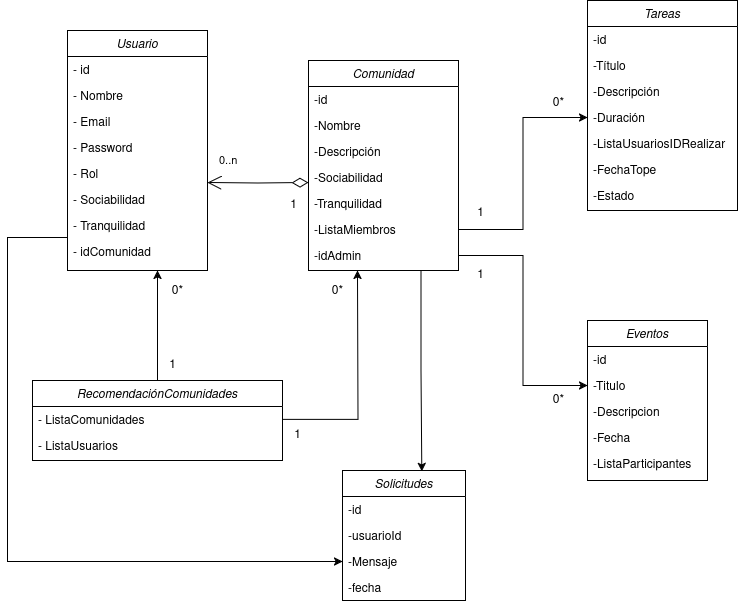
\includegraphics[width=\textwidth]{fotos/TFG1-Page-6.drawio(3).png}
    \caption{Diagrama UML de clases de análisis.}
\end{figure}
